\chapter{Trabalhos Relacionados}\label{cap:relacionados}
Em busca de trabalhos que visam o desenvolvimento de aplicações para o auxílio ao tratamento de crianças com transtorno do espectro autista, cinco artigos e cinco aplicativos se destacam por terem a mesma finalidade ou finalidades similar ao tema.


\section{Artigos}
\begin{itemize}
	\item O trabalho proposto por \citeonline{neto2017cotidiano}, apresenta a proposta de um software para auxiliar as crianças autista em suas atividades de vida diária, visto que essa é uma das maiores dificuldades apresentadas. O software em questão tem como objetivo dar mais autonomia e inclusão a pessoas com transtorno do espectro autista, de níveis leves e moderados.
	
	O aplicativo de \citeonline{neto2017cotidiano} funciona com atividades básicas que o próprio autista pode escolher fazer, como: ir ao banheiro, comer, beber ou brincar, e com atividades que são previamente agendadas, como acordar: almoçar, estudar, jantar e dormir, sendo que todas essas atividades são cadastradas e gerenciadas pelo responsável da criança com TEA.
	
	\item \citeonline{farias2013prototipo}, em seu trabalho apresenta os resultados parciais no processo de elaboração de um software, que será usado para a alfabetização de crianças com TEA, usando para isso o método TEACCH, o qual é amplamente utilizado e bastante comprovado no tratamento.
	
	A ideia do software proposto por \citeonline{farias2013prototipo}, é de que haja a possibilidade de o profissional crie atividades que serão executadas posteriormente pelas crianças, sendo que é possível que o profissional acompanhe a evolução da criança.
	
	\item O trabalho proposto por \citeonline{cartagenes2017software}, apresenta o desenvolvimento de um jogo, que tem por nome \textit{MOTIVAeduca}, que trabalha com a técnica ABA, a qual é bastante aplicada durante os tratamento convencionais.
	
	\citeonline{cartagenes2017software}, tinham como objetivo, desenvolver  as mesmas atividades que eram realizadas convencionalmente de forma manual, porém, de uma maneira virtual. Eles partiram do principio que as crianças são aprendizes primariamente visuais, com isso, é uma forma de ajuda-las a se comunicarem  e expressarem, o aplicativo \textit{MOTIVAeduca} tenha que associar formas a imagens, animais a seus alimentos e por fim, completar figuras.
	
	\item O trabalho apresentado por \citeonline{aziz2014educational}, mostra o processo de desenvolvimento de um aplicativo para a plataforma IOS, e é focado na solução de comunicação verbal, o aplicativo dá uma forma de a criança com TEA, expressar seus desejos em forma de dialogo, o aplicativo permite com que a criança selecione e escolha o que precisa.
	
	\item O trabalho apresentado por \citeonline{ern2014use}, tem como objetivo o estudo e revisão de formas para dar interação a crianças com o transtorno do espectro autista, através do uso de técnicas de gamificação.
	
	\citeonline{ern2014use} realizou sua pesquisa bibliográfica com o uso de quatro bases de dados, sendo elas: \textit{PsychInfo, SciVerse Scopus, ScienceDirect e Web of Knowledge}. Os autores buscaram artigos que tinha relação com o tema de jogos na atenção a saúde e por fim eles aplicaram um processo de triagem para realizar a filtragem para os trabalhos que falassem exatamente da gamificação para o autismo, restando no fim apenas 14 artigos de um total de 4556.
	
	Como resultado \citeonline{ern2014use}, montou uma tabela com os aplicativos propostos nos artigos e com isso ele consegue classifica-los de acordo com suas características e elementos de jogo que ele chamou de \textit{Ingredientes de Grandes Jogos}. Também conseguiu montar uma tabela com informações importantes daquele jogo ou intervenção, como : nome, tecnologia, materiais de apoio, grupo alvo e eficácia.
\end{itemize}

\section{Aplicativos}

Foram realizadas pesquisas na loja de aplicativos da plataforma android, em busca de aplicativos que seguissem o mesmo foco apresentado neste trabalho, são eles:

%\begin{figure}[H]
%	\centering
%	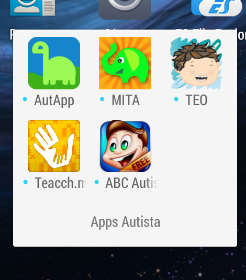
\includegraphics[scale=0.5]{img/appsRelacionados.png}
%	\caption{Aplicativos Relacionados}
%	Fonte:Autor, 2018
%\end{figure} 

\begin{itemize}
	\item \textit{AutApp}\footnote{AutApp pode ser baixado através do link: https://bit.ly/2sOKU50}. Se encontra na conta de Gabriel Hahn Schaeffer, segundo a descrição na própria loja, o aplicativo se trata do TCC de um aluno do curso de engenharia da computação.
	
	O aplicativo se divide em duas partes, são elas: 	
	\begin{itemize}
		\item A primeira que se chama \textit{O Que o Erick Está Sentindo} que consiste em uma imagem mostrada, do personagem Erick com uma expressão e ao clicar em responder são mostrados o Erick com quatro expressões, na qual a criança deve escolher qual a que foi mostrada.
		
		\item O segundo item, chamado  \textit{Vamos Brincar}, trata-se da associação de figuras e suas respectivas sombras, na qual a criança com autismo deve relacioná-las.
	\end{itemize}
	\item \textit{MITA}\footnote{MITA pode ser baixado através do link: https://bit.ly/2JhZ4q5}. Se encontra na conta da ImagiRation LLC , segundo a descrição presente lá o MITA desenvolve a capacidade de integração e as funções mentais da criança.
	
	O aplicativo apresenta uma séries de desafios, na qual a criança deve cumprir, sendo estes voltados para a associação de imagens e memorização, os desafios são divididos por fases e ao cumprir todas essas fases é dado uma recompensa à criança.
	
	\item \textit{TEO}\footnote{TEO pode ser baixado através do link: https://bit.ly/2JnsoMg}.  Se encontra na conta de Thiago Bruno Melo de Sales, segundo a descrição na própria loja, TEO é um acrônimo para Tratar, Estimular e Orientar, foi desenvolvido por alunos e pesquisadores do curso de Ciência da Computação da Universidade Federal de Alagoas.
	
	O aplicativo abrange diversas atividades como a associação de cores, numéricas, quebra cabeça, atividades diárias na qual o aplicativo da uma foto do rosto de uma pessoa e pergunta onde está tal elemento do rosto, e a criança deve clicar no lugar que ela acha que é o elemento mostrado. E por fim, é possível visualizar uma tela onde se encontram estatísticas sobre os jogos realizados pela criança.
	
	
	\item \textit{Teacch.me}\footnote{Teacch.me pode ser baixado através do link: https://bit.ly/2yflNwE}. Se encontra na conta de Leonardo Felipe Nerone e segundo a descrição na própria loja o aplicativo é completamente baseado no método de tratamento TEACCH.
	
	No aplicativo é possível que o responsável defina atividades que a serem realizadas pela criança, podendo definir um horário ou, simplesmente, usar das atividades que o próprio aplicativo disponibiliza. O aplicativo conta também com uma sessão de perguntas frequentes sobre o autismo para auxiliar aos responsáveis.
	
	\item \textit{ABC autismo}\footnote{ABC Autismo pode ser baixado através do link: https://bit.ly/1NsObMf}.  Se encontra na conta de Dokye Mobile e segundo a descrição na própria loja, o aplicativo se baseia em metodologias TEACCH e contempla quatro níveis de dificuldade, possui 40 fases interativas, estrelas para colecionar e está disponível em português, inglês e espanhol.
	
	O jogo consiste basicamente em quatro níveis, onde a dificuldade é aumentada de acordo com o nível,os níveis consistem basicamente em associações de objetos com contornos, sombras e objetos semelhantes.
\end{itemize}

\section{Considerações Finais}
Tendo em vista os trabalhos apresentados ao longo dessa seção, considera-se que o trabalho objetivo desta pesquisa tem algumas características em comum com alguns deles, porém, em nenhum foi observado a interação entre o profissional, paciente e pais, e outra característica que o difere dos demais é a possibilidade de tanto os pais quanto os profissionais possam acompanhar o desenvolvimento da criança com o ranking geral de pacientes para o profissional, onde é possível ver todos os pacientes, classificados por pontos, e o profissional pode ver o avanço de seu filho de acordo com as pontuações e níveis.